\documentclass[10pt,a4paper]{article}
\usepackage[utf8]{inputenc}
\usepackage[T1]{fontenc}
\usepackage{amsmath}
\usepackage{amssymb}
\usepackage{graphicx}
\usepackage[english]{babel}
\usepackage{float}
\usepackage{geometry}
\geometry{top=1cm}
\title{Assignment \#8}
\author{Soulimane Mammar}
\begin{document}
	\maketitle
	\section*{Exercise 1}
	Create a class \verb|FLOAT| that contains one \verb|float| data member. Overload all the four arithmetic operators so that they operate on the objects of \verb|FLOAT|.
	\section*{Exercise 2}
	Design a class \verb|Polar| which describes a point in the plane using polar coordinates \verb|radius| and \verb|angle|. A point in polar coordinates is shown in the following figure
	\begin{figure}[H]
		\centering
		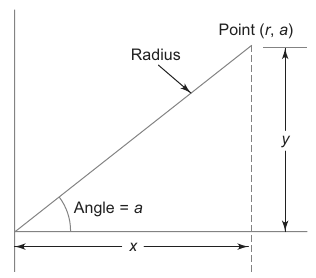
\includegraphics[width=0.5\linewidth]{polar_coordinates}
	\end{figure}
	\noindent Use the overloaded \verb|+| operator to add two objects of Polar. 
	
	\noindent Note that we cannot add polar values of two points directly. This requires first the conversion of points into rectangular coordinates, then adding the corresponding rectangular coordinates and finally converting the result back into polar coordinates. You need to use the following trigonometric formulae:
	\begin{verbatim}
		x = r * cos(a); 
		y = r * sin(a); 
		a = atan(y/x); // arc tangent 
		r = sqrt(x*x + y*y); 
	\end{verbatim}
	
	\section*{Exercise 3}
	Create a class \verb|MAT| of size m $\times$ n. Define all possible matrix operations for \verb|MAT| type objects.
	
\end{document}